\documentclass[11pt, a4paper]{article}

\usepackage[utf8]{inputenc}
\usepackage[T1]{fontenc}
\usepackage[spanish, es-nodecimaldot]{babel}
\usepackage{graphicx}
\usepackage[top=2.2cm, bottom=2.5cm, left=2.2cm, right=2.2cm]{geometry}
\usepackage{caption}
\usepackage{float}
\usepackage{microtype}
\usepackage{booktabs}
\usepackage{amsmath}
\usepackage{textcomp}
\usepackage{xcolor}
\usepackage{array}
\usepackage{tabularx}
\usepackage{xurl}
\usepackage[colorlinks=true, linkcolor=blue!70!black, urlcolor=blue!70!black, citecolor=blue!70!black]{hyperref}
\graphicspath{{../output/figures/}}
\captionsetup{font=small, labelfont=bf, justification=centering}
\setlength{\emergencystretch}{2em}

\title{\textbf{Trabajo Práctico 8: Población, Género y Desarrollo}\\[0.3em]
\large Evidencia Empírica para la India}
\author{
    \footnotesize \textbf{Mateo Barros} \quad \textbf{Felipe Delgado} \quad \textbf{Santiago González} \quad \textbf{Rodrigo Stremel} \quad \textbf{Santiago Trivellini} \\[0.3em]
    \footnotesize \textit{Desarrollo Económico --- Licenciatura en Economía --- Universidad Nacional del Sur (UNS)}
}
\date{\small Octubre de 2026}

\begin{document}
\maketitle
\vspace{-1em}
\noindent\rule{\textwidth}{0.6pt}
\vspace{0.8em}

\section{Población}

\subsection{Crecimiento poblacional}

La tasa natural de crecimiento de la población es distinta a la tasa de crecimiento de la población ya que esta última contiene el factor de la migración neta.

\begin{figure}[H]
\centering
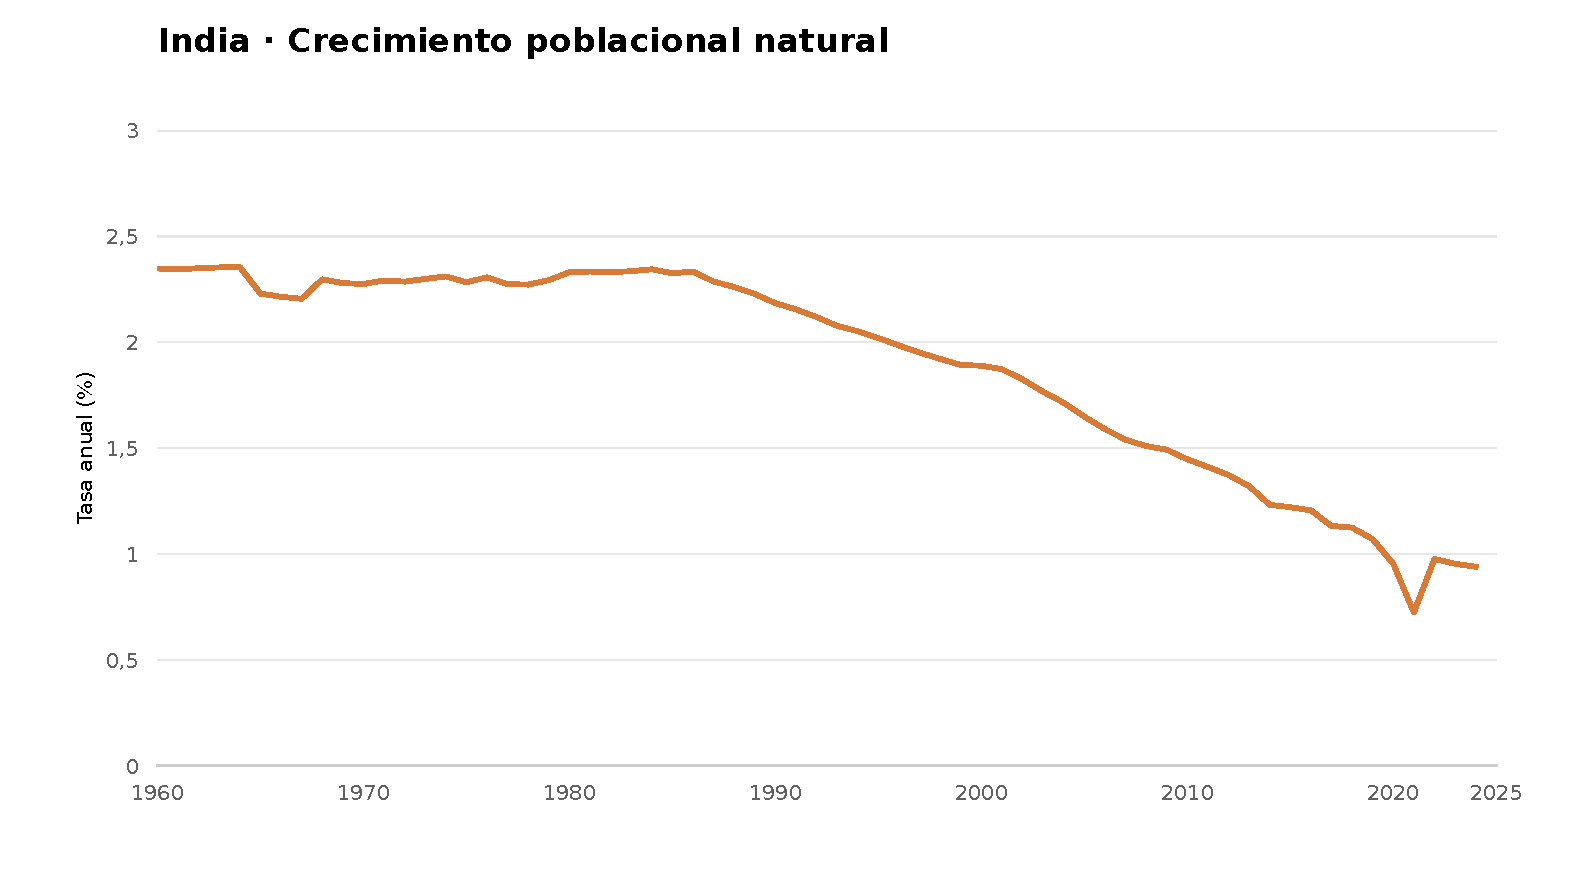
\includegraphics[width=0.96\textwidth,height=0.43\textheight,keepaspectratio]{02_crecimiento_poblacional_natural.pdf}
\caption{India: tasa natural de crecimiento poblacional.}
\label{fig:crecimiento_natural}
\end{figure}

La India continúa con un crecimiento natural de la población, aunque a ritmos considerablemente menores que a mitad del siglo pasado.  Como grupo, desde el desconocimiento, no esperábamos una caída tan abrupta en la tasa, aunque el signo positivo era predecible.

Nos pareció interesante comparar el dato con la tasa de crecimiento poblacional neto, ya que la India cuenta con una fuerte tendencia a la migración. Como suponíamos, tienden a ser similares puesto que se compensa la gran masa migratoria con el crecimiento poblacional natural.

\begin{figure}[H]
\centering
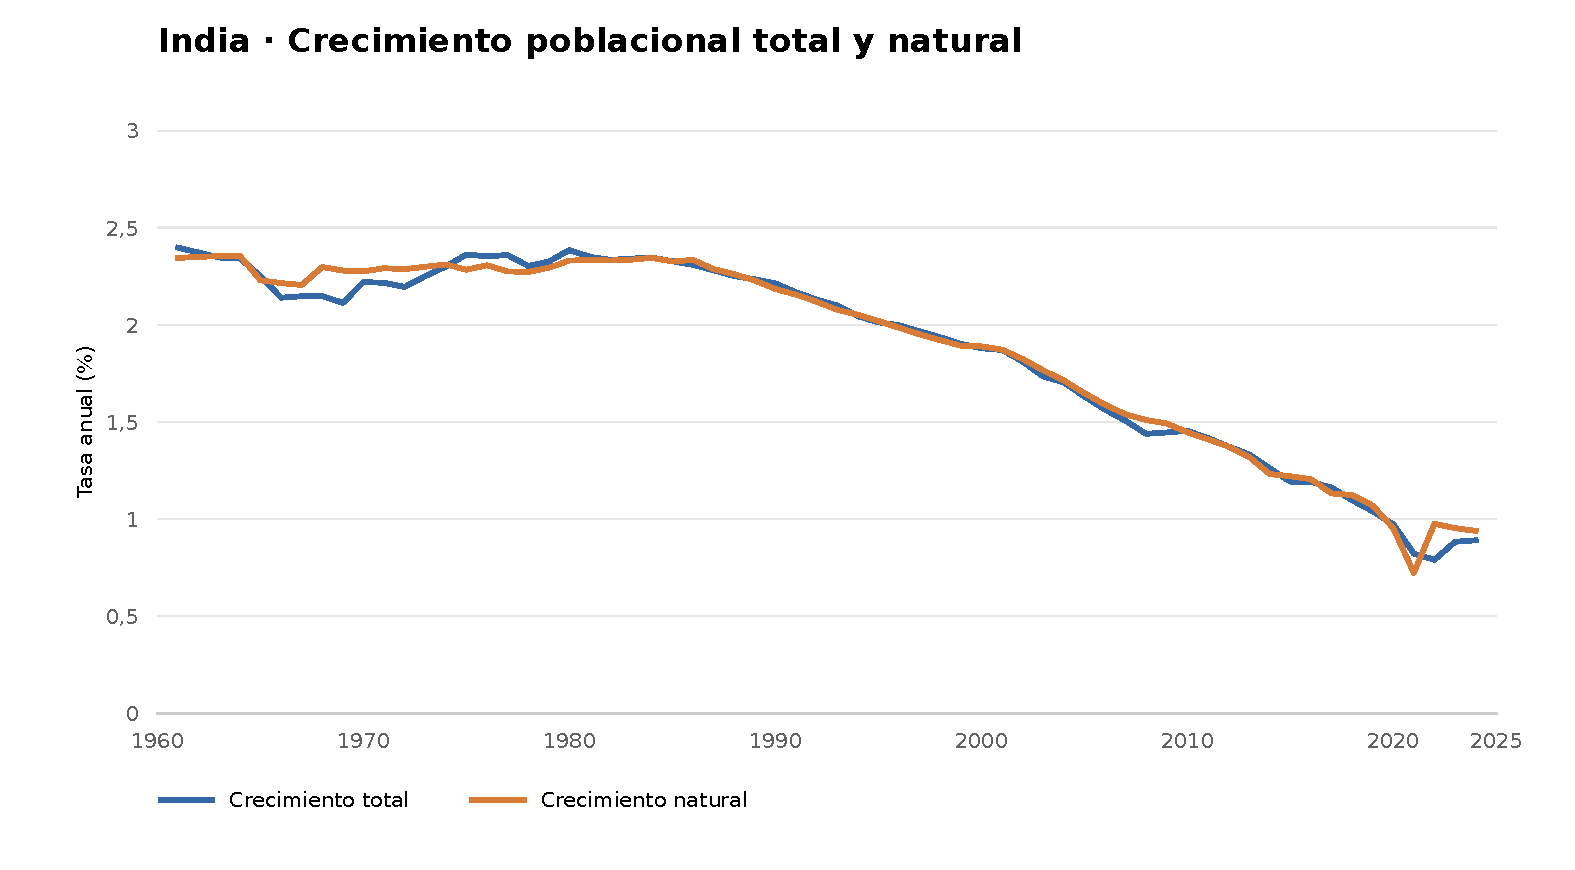
\includegraphics[width=0.96\textwidth,height=0.43\textheight,keepaspectratio]{03_crecimiento_total_y_natural.pdf}
\caption{India: crecimiento poblacional total y natural.}
\label{fig:total_natural}
\end{figure}

\subsection{Transición demográfica}

\begin{figure}[H]
\centering
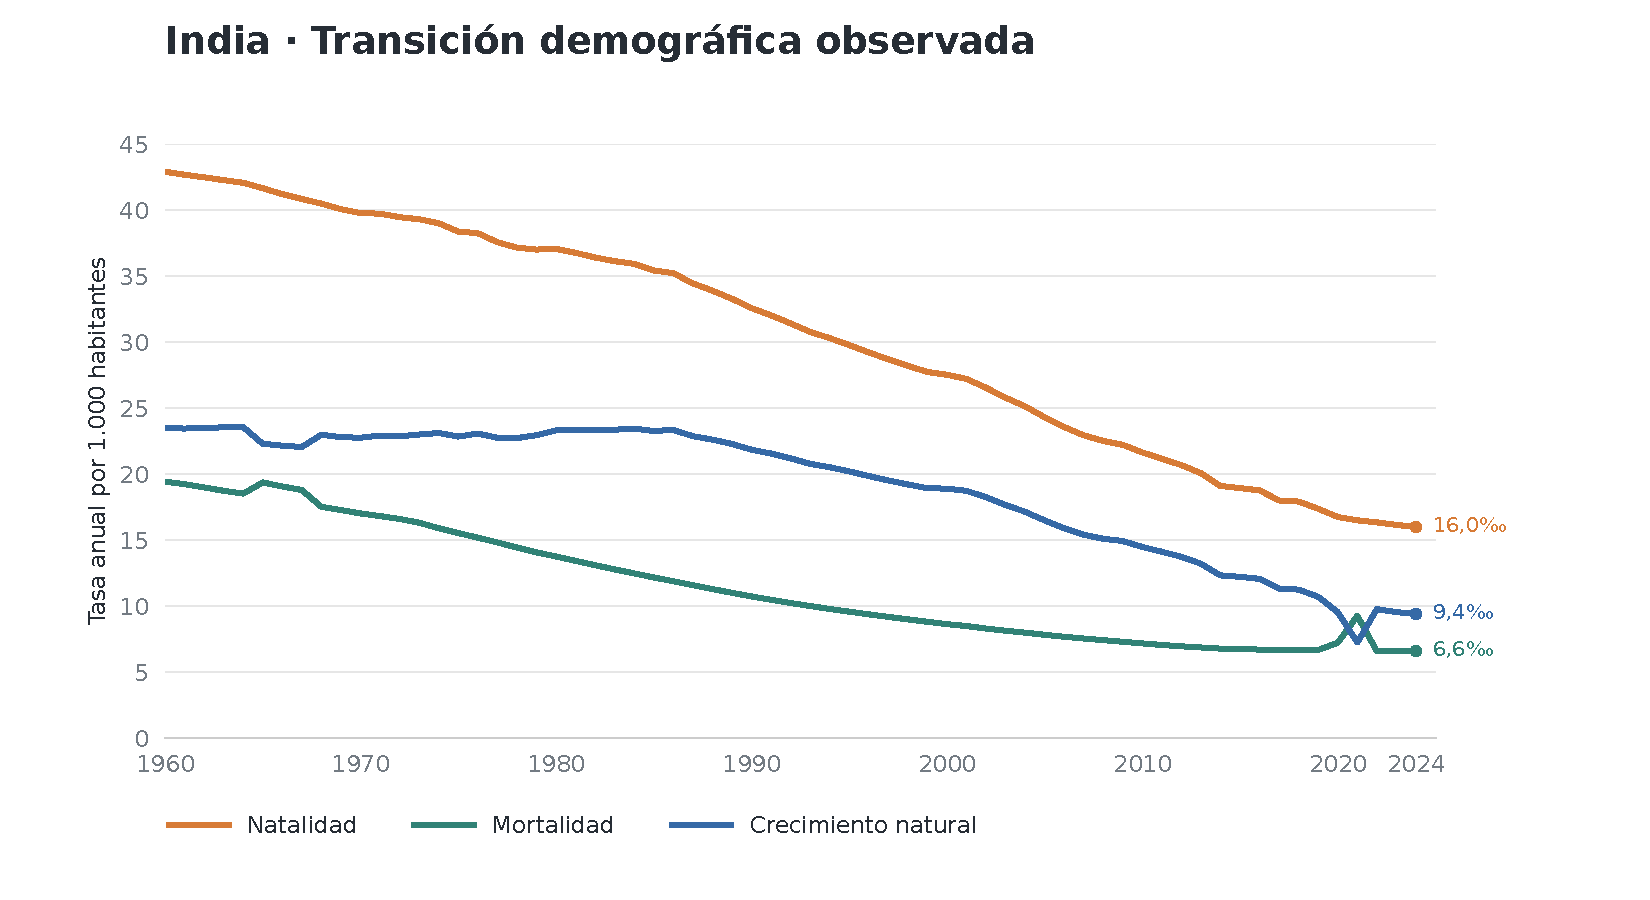
\includegraphics[width=0.96\textwidth,height=0.43\textheight,keepaspectratio]{05_transicion_demografica_datos_india.pdf}
\caption{India: evolución observada de natalidad, mortalidad y crecimiento natural.}
\label{fig:transicion_observada}
\end{figure}


En el caso de India, observamos una desaceleración tanto en la tasa de mortalidad como en la tasa de mortalidad resultando en una reducción del porcentaje de crecimiento poblacional natural.  Siguiendo la teoría, la ubicamos en el final de la fase 3, realizando la transición hacia la etapa 4, donde la natalidad y la mortalidad se mantienen bajas y el crecimiento natural tiende a estabilizarse en niveles reducidos.

Ilustrativamente:

\begin{figure}[H]
\centering
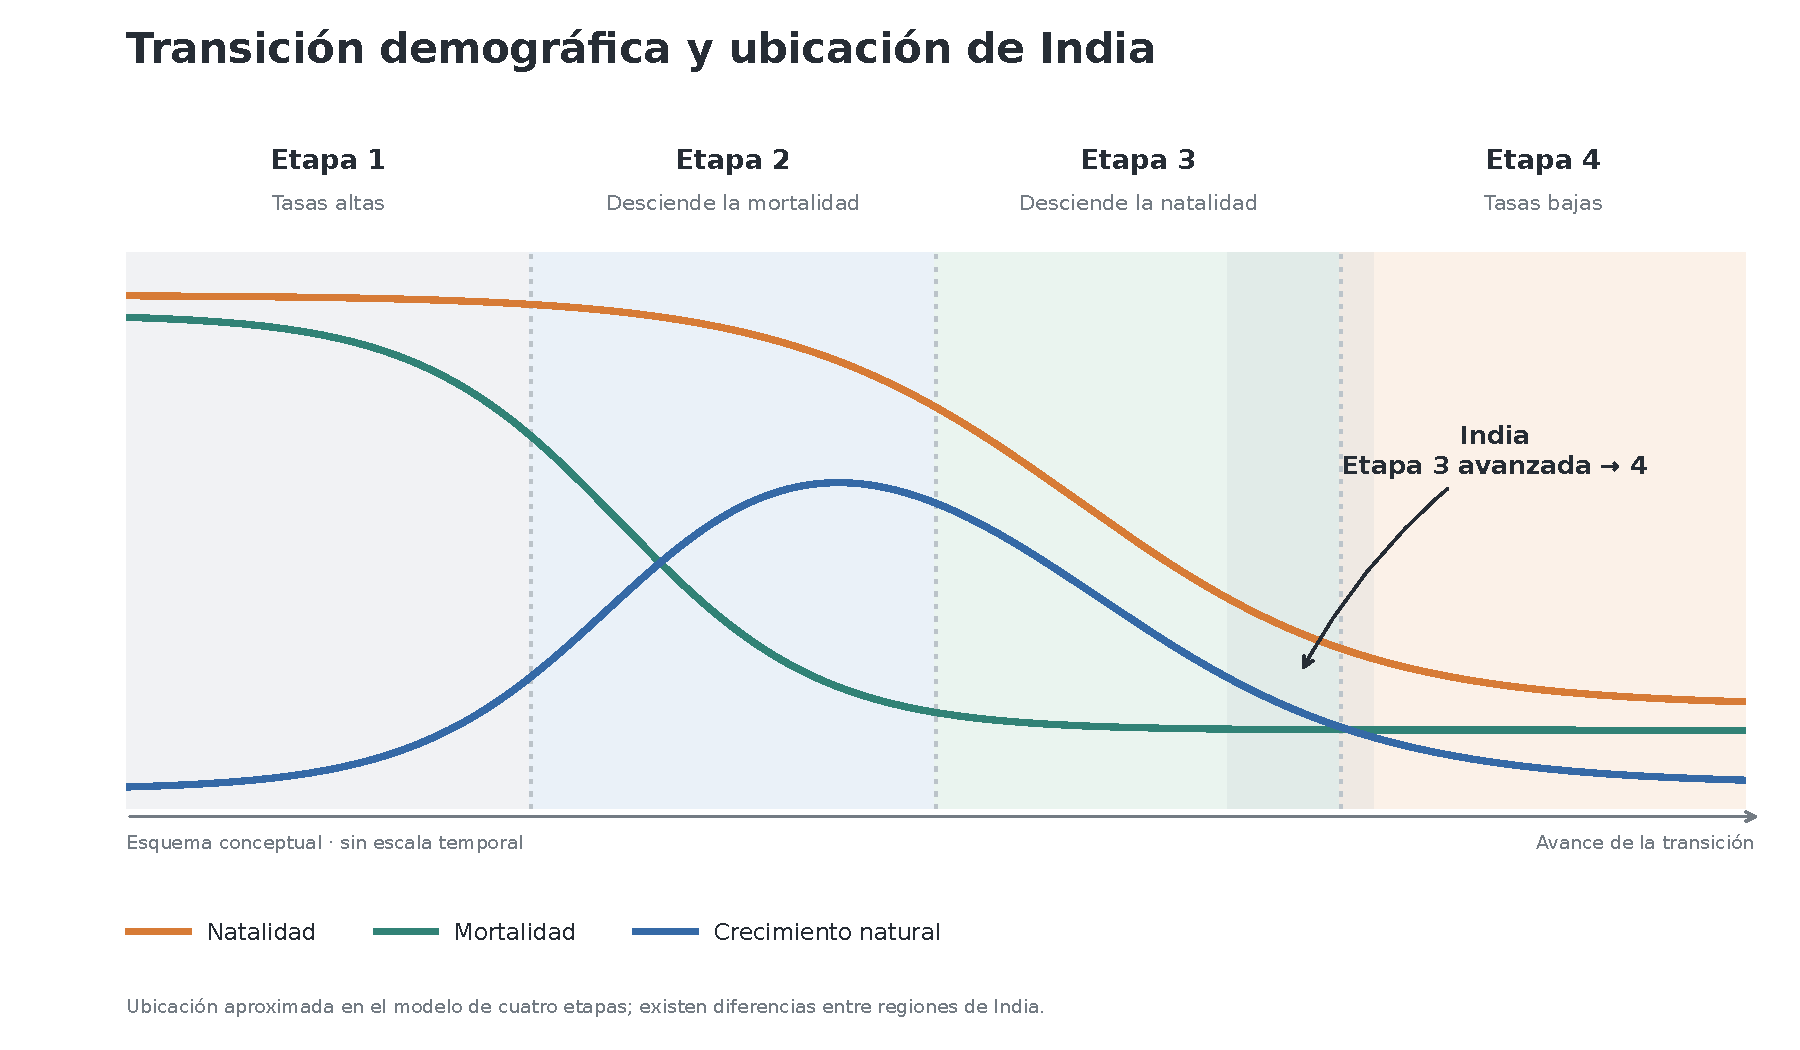
\includegraphics[width=0.96\textwidth,height=0.43\textheight,keepaspectratio]{04_transicion_demografica_esquema.pdf}
\caption{Esquema conceptual de la transición demográfica y ubicación aproximada de India.}
\label{fig:transicion_esquema}
\end{figure}


\subsection{Índice de dependencia}

\[
\text{Índice de dependencia} =
\frac{\text{Población hasta 15 años} + \text{Población de más de 65 años}}
{\text{Población entre 15 y 65 años}}.
\]

\begin{figure}[H]
\centering
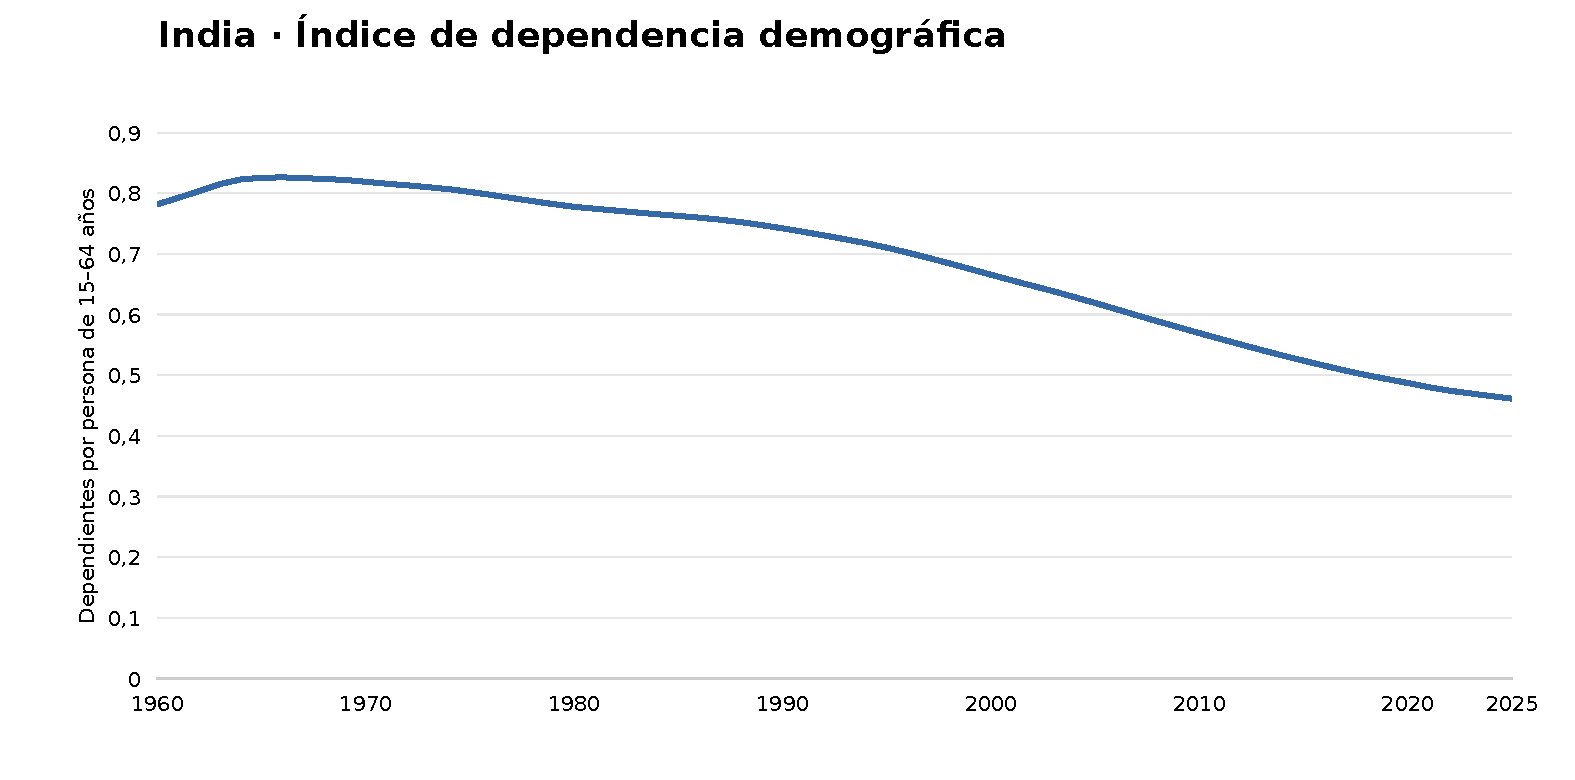
\includegraphics[width=0.96\textwidth,height=0.43\textheight,keepaspectratio]{06_indice_dependencia_india.pdf}
\caption{India: índice de dependencia demográfica, expresado como razón.}
\label{fig:dependencia}
\end{figure}

\subsection{Bono demográfico}

India es el país con más habitantes del planeta, figurando aproximadamente una población de 1480 millones. Cuya tasa de natalidad se encuentra en descenso.

El dividendo demográfico reporta una edad  promedio de 29 años, que se puede traducir en beneficios en términos de productividad económica, que permitirá contar con un porcentaje esperado muy alto de personas en edad activa en los próximos años, esto teniendo en cuenta que todos los estudiantes tengan acceso a una orientación que vaya más allá de la educación tradicional.

Sin embargo, el alto bono demográfico que a corto plazo puede ser una buena noticia, considerando la disminución de la tasa de natalidad en los últimos años, puede que a  largo plazo se genere una reversión en la población joven actual, a un masivo porcentaje de gente adulta. En las próximas décadas se espera que la India tendrá una mayor proporción de personas mayores y, con el tiempo, una menor proporción de personas en edad laboral. Corre el riesgo de ``envejecer'' sin crecer o desarrollarse.

\subsection{Migración neta y remesas}

En el caso de India existe emigración neta, es decir, los migrantes superan a los inmigrantes (podemos llamar a este concepto: migración neta negativa). Es decir, existe una mayor cantidad de personas que se marchan del país dirigiéndose hacia otro país para vivir en comparación a la cantidad de personas que llegan y se mudan al país.

Una de las ventajas que posee gozar de emigración neta consiste en las remesas (transferencias monetarias de indios que migraron hacia otro país y envían dinero a, por ejemplo, familiares). La segunda ventaja visible reside en que, al reducir la cantidad de personas para una misma cantidad de recursos, disminuye la escasez de bienes y recursos útiles para la sociedad (de todo tipo, desde alimentos hasta viviendas) mejorando relativamente las posibles condiciones de vida.

Yendo a los datos, podemos comparar las remesas con otras fuentes de entradas de divisas, por lo que utilizaremos: Remesas como \% del PBI, Exportaciones como \% del PBI e IED como \% del PBI.

\begin{figure}[H]
\centering
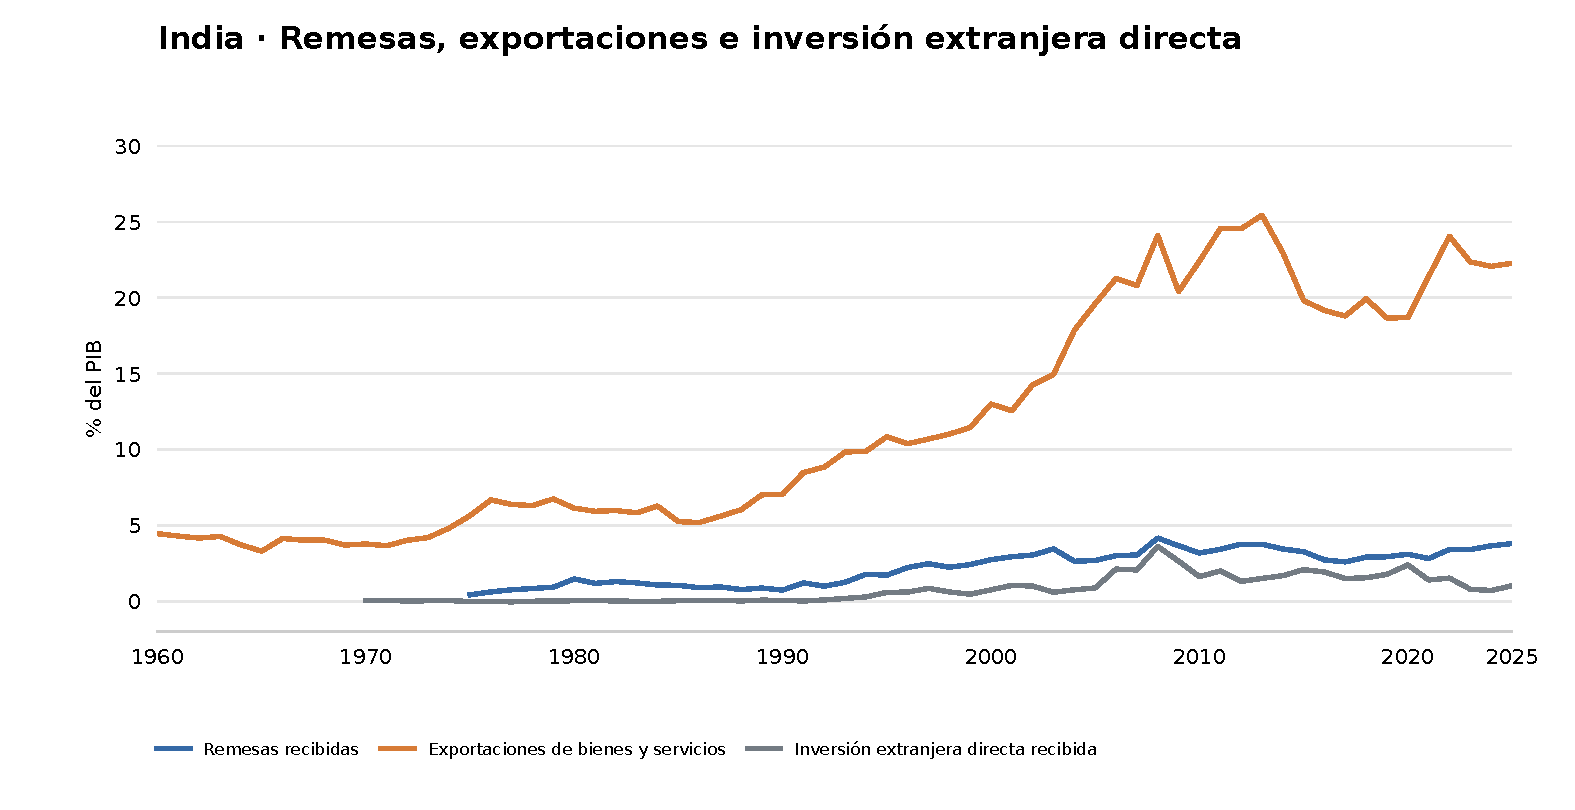
\includegraphics[width=0.96\textwidth,height=0.43\textheight,keepaspectratio]{07_remesas_exportaciones_ied.pdf}
\caption{India: remesas, exportaciones e inversión extranjera directa como porcentaje del PIB.}
\label{fig:remesas}
\end{figure}

A pesar de no contar con ciertos años, observando los datos entendemos que, para India, la importancia de las remesas (con un promedio de 1,16\% a lo largo del tiempo) recibidas para el desarrollo del país fue decayendo a partir de los 80s. Como cabía suponer, se evidencia una dominancia clara por parte de las exportaciones (con un promedio de 10,8\% a lo largo de la serie) mientras que el segundo lugar -de este gráfico- fue en un primer momento para las remesas, que luego fueron superadas por la Inversión Extranjera Neta (con un promedio de 0.98\% en la serie completa).

En conclusión, actualmente las remesas no representan una porción significativa y esencial del PBI Indio y mucho menos para el desarrollo en general, por lo que su economía no pareciera depender de las transferencias de los migrantes sino de otras cuestiones, como por ejemplo las exportaciones de bienes y servicios.


\section{Género}

\subsection{Evolución de la desigualdad de género}

\begin{figure}[H]
\centering
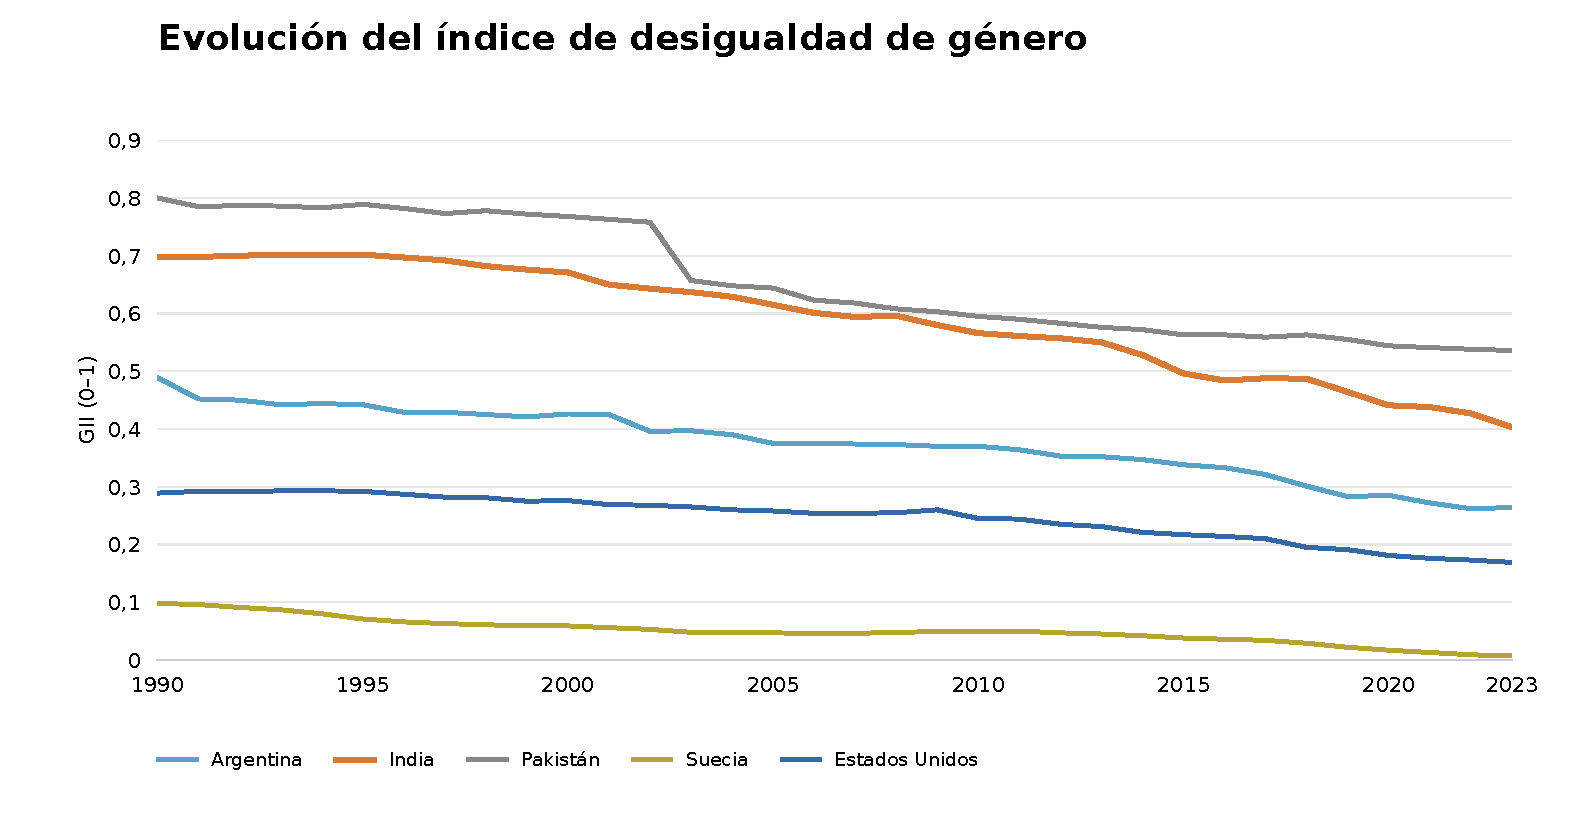
\includegraphics[width=0.96\textwidth,height=0.43\textheight,keepaspectratio]{08_gii_comparacion_paises.pdf}
\caption{Evolución del índice de desigualdad de género en los cinco países seleccionados.}
\label{fig:gii}
\end{figure}

Analizando el gráfico, se ve una tendencia global negativa en el índice, lo que se traduce a una reducción mundial de la desigualdad de género.

Si bien esta tendencia demuestra avances en la integración, se evidencia que India todavía tiene un gran margen de mejora, ya que continúa siendo de los países con mayor desigualdad en el mundo, ocupando el lugar 102 en el mundo


\subsection{Comparación de indicadores}

\begin{table}[H]
\centering
\small
\caption{GII y componentes en Argentina, India y Estados Unidos.}
\label{tab:gii_comparacion}
\renewcommand{\arraystretch}{1.25}
\begin{tabularx}{\textwidth}{>{\raggedright\arraybackslash}Xrrr}
\toprule
\textbf{Indicador} & \textbf{Argentina} & \textbf{India} & \textbf{Estados Unidos} \\
\midrule
Natalidad adolescente (nacimientos por 1.000 mujeres de 15--19 años) & 26,41 & 14,06 & 13,15 \\
Índice de desigualdad de género (GII, de 0 a 1) & 0,26 & 0,40 & 0,17 \\
Posición en el ranking del GII & 70 & 102 & 45 \\
Participación laboral de mujeres de 15 años o más (\%) & 53,16 & 35,08 & 57,33 \\
Participación laboral de varones de 15 años o más (\%) & 72,22 & 76,41 & 68,12 \\
Razón de mortalidad materna (muertes por 100.000 nacidos vivos) & 44,90 & 102,65 & 21,09 \\
Bancas parlamentarias ocupadas por mujeres (\%) & 43,77 & 14,82 & 28,22 \\
Bancas parlamentarias ocupadas por varones (\%) & 56,23 & 85,18 & 71,78 \\
Mujeres de 25 años o más con al menos parte de educación secundaria (\%) & 74,30 & 43,50 & 97,87 \\
Varones de 25 años o más con al menos parte de educación secundaria (\%) & 72,22 & 61,09 & 97,83 \\
\bottomrule
\end{tabularx}
\end{table}


Si bien India se encuentra peor en cada aspecto del índice respecto de Argentina y Estados Unidos, en donde se ve mas diferencia es en el radio de mortalidad materna (razón de mortalidad materna, donde más que duplica a Argentina y casi que quintuplica a Estados Unidos), el porcentaje de sillas del parlamento que son ocupadas por mujeres (participación de mujeres en el parlamento) y en el porcentaje de mujeres de más de 25 años que terminaron el secundario (población femenina con al menos parte de educación secundaria).

Estos problemas no se solucionan con crecimiento, y hasta pueden incrementarse, si no que se corrigen por medio de las instituciones. Un claro ejemplo es en la comparación de Argentina contra Estados Unidos en la dimensión de participación de mujeres en el parlamento, donde Argentina que es un país con menor poderío económico que Estados Unidos, tiene casi el doble de porcentaje de mujeres en el parlamento, lo cual se debe a leyes de Argentina que garantizan los puestos de mujeres

\end{document}
